% Ian Wilkes 
% Artificial Intelligence 600.335
% Assignment 4.
\documentclass[12pt, letterpaper]{article}
\usepackage{amsmath, amsthm, graphicx}


\title{Decision Trees for Classification: \\ An Evolutionary Approach}

\author{Ian Wilkes}

\begin{document}

\maketitle

\begin{abstract}
Classification is one of many extremely important topics within the field of 
artificial intelligence, and is used in many fields from advertising to 
quality control.  As such it is imperative that we be able to provide efficient
and accurate classifiers. One such method for classification is through the use
of decision trees.  This paper will discuss two implementations of decision trees, one using information gain, and another which evolves to learn to classify
sets of data.  Their comparative performance will be discussed, as well as 
ways to optimize each of their individual performance. 


\end{abstract}

\section{Introduction}

\section{Learning Decision Trees}
\subsection{Information-Theoretic Methods}
\subsubsection*{Entropy and Information Gain}
\subsection{Genetic Algorithms}

\subsubsection*{Genetic Algorithms for Decision Trees}

\section{Algorithms and Experimental Methods}

\subsection*{Data Sets}

\section{Results}
\begin{figure}[!htb]
\begin{center}
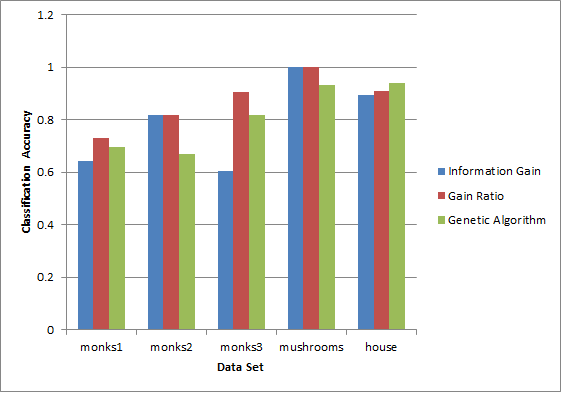
\includegraphics[width=4in]{images/algorithm_comparison_accuracy.png}
\end{center}
\caption{This figure shows the classification accuracy of the information gain
based, gain ratio, and genetic decision trees.  It can be seen that the gain 
ratio based tree seems to perform the best in almost all cases.}
\label{Classification Accuracies of Multiple Decision Trees}
\end{figure}

\begin{figure}[!htb]
\begin{center}
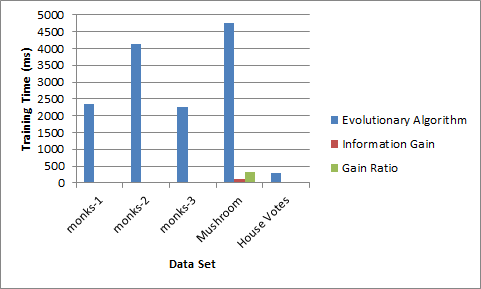
\includegraphics[width=4in]{images/algorithm_comparison_training_time.png}
\end{center}
\caption{This figure shows the required training times of the information gain
based, gain ratio, and genetic decision trees.  It can be seen that the genetic
tree takes much more time than either of the other trees.}
\label{Training Times of Multiple Decision Trees}
\end{figure}

\begin{figure}[!htb]
\begin{center}
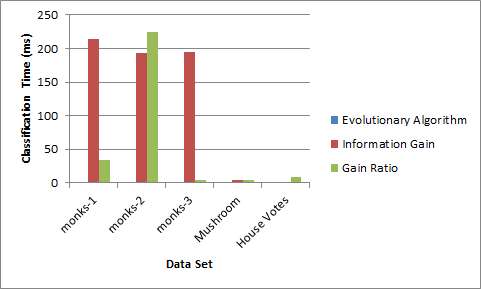
\includegraphics[width=4in]{images/algorithm_comparison_testing_time.png}
\end{center}
\caption{This figure shows the testing time of the information gain
based, gain ratio, and genetic decision trees.  Here, the evolutionary or 
genetic tree takes orders of magnitude less time than the information based
trees.}
\label{Testing Times of Multiple Decision Trees}
\end{figure}



\begin{table}
\begin{center}
\begin{tabular}{|c||c|cc}
\hline
& col1 & col2 & col3\\
\hline \hline
row1 & a & b & c\\
\hline 
row2 & d & e & f\\
\hline 
row3 & g &   & h\\
 & i & j & k\\
\hline 
\end{tabular}
\end{center}
\caption{This is a caption on the table.  Try to keep your captions short; don't
put multiple paragraphs of text in here.  Put the long version in the Results
section, and reference the table from there.}
\label{sometable}
\end{table}
From figure 1 we can see that the performances of the genetic, information
gain and gain ratio based trees are all somewhat comparable.  The gain ratio
tree seems to perform the best of the three in all but the house votes data set.
It drastically out performs the information gain based tree on the monks-3 data
set, whcih is also beaten by the genetic algorithm.

Moving on to figure 2, it is plain to see that the evolutionary algorithm
takes much longer to train than the traditional decision trees, neither of which
ever takes even 500ms to train, while the genetic tree takes almost 5000ms on 
the mushroom data set.

The opposite trend can be seen in the classification times of the testing sets,
which can be observed in figure 3.
The information gain and gain ratio trees take orders of magnitued more time
to classify their data on the monks-1, monks-2, and monks-3 data sets than the
genetic tree.


The results section should contain your results.  It should \emph{not} contain
your interpretation of those results.  That comes later.  This section should be
made up primarily of graphs and tables that show your data.  You should also
have a small amount of text describing what each of the tables and graphs shows,
since the caption on the figures should be short.  Having text describing the
specifics of the experiment that lead to that particular table would also be
good.  For example,

\begin{quote}
``Table \ref{sometable} shows the average results of the three algorithms on all
the data sets.  The parameters used were $N=7$, and $k=3.27$; these parameters
were found by hand, and little effort was made to tune them optimally.  Each
algorithm was run three times on each of the seven data sets, and the resulting
accuracy scores were averaged.''
\end{quote}

I'm not going to tell you exactly what tables or graphs you should have here,
since it will depend a bit on your results.  You should be sure that your
results section contains sufficient data to support your conclusions about the
relative strengths and weaknesses of the different algorithms.  You should also
be sure that your data is complete; that is, don't leave data out simply because
it doesn't support the point you're trying to make.

You should also be sure that your results are clear and interpretable.  Seven
pages of raw binary data will do nothing to edify your reader.  Similarly, a
1 inch square graph with 12 lines plotted on it will be difficult to extract
meaning from, as will a graph with poor (or no) labels on the axes.  Your
results should be legible both on screen and in hard copy.

You don't want to present results that are just raw data, since that is hard to
interpret.  But you don't want to over abstract, either, since that leads to
results that have little or no meaning (eg. ``the average over all different
data sets, algorithms, and parameters'' is a completely useless statistic for
comparing algorithms).

If you are trying do draw comparisons between certain things, try to make sure
your results are presented in a way that allows the reader to easily compare
them.  This might mean having two lines in the same graph, or it might mean
having the columns you want to compare be adjacent in a table.  You want it to
be easy for the reader to follow whatever reasoning you make in your Conclusions
section by looking at your Results.  You don't want to redundancy (don't put the
same data in multiple different tables), but you want the reader to be able to
evaluate your conclusions without having to compare things that are three pages
apart in your Results.

You should probably have a page or two of results; one or two tables are unlikely to be
sufficient to describe your experiments.  If they are, you need to do more
experiments.  On the other hand, if you have more than three pages, you're
probably not doing a good job of presenting your data in a clear and concise
form.

\section{Discussion}
The discussion section is where you discuss your interpretation of the data you
presented in the results section.  This is where you tell the reader how great
your algorithm is, and how interesting it is that \emph{this} performed better
than \emph{that} on some given data set.  You can also speculate about causes
for interesting behaviors; for example, if you think you might know why it fails
so badly on some particular case, or if you have an insight into why it did well
on another case.  You don't want to be making wild guesses, but as long as you
make it clear that you are not making claims of factual proof, you can go out on
a limb a little.  For example,

\begin{quote}
``In most cases, algorithm A outperforms algorithm B with a significance of
99.8\%.  However, as can be seen from Figure \ref{somefigure}, when applied to
the ``E. E. Smith'' data set, algorithm A does no better than random chance.  It
seems likely that the failure of algorithm A to learn is due to the extremely
sparse distribution of that data set.  Because of algorithm A's heavy reliance
on data being densely sampled from the true underlying distribution, any sparse
data set is likely to show this behavior.''
\end{quote}

Think about the kinds of questions that were posed in the written portions of
homework assignments 1 and 2; these are the kinds of things you want to think
about for your Discussion.

\section{Conclusions}
The conclusion section should be relatively short, and should not be a summary
of your paper.  It should, however, bring up what you learned and what impact
your results have on the rest of the field (and society as a whole, if
applicable, but don't overstate the impact of what you're doing).  You should
conclude, and bring your paper to an end with any parting thoughts that are
appropriate.

Certain types of papers can be ended with a ``Summary'' section instead of a
``Conclusions'' section, in which case you would, in fact, summarize the main
points of your paper.  For this paper, you should write a Conclusions section,
not a Summary.

Conclusion also often contain information about what else you would like
to do.  Sometimes this is a separate subsection, or even a section, entitled
``Future Work.''  The basic idea here is to talk about what the next steps to
take would be.  This is of benefit to others who are interested in your
work and may want to help advance it.  It is also a chance for you to
acknowledge shortcomings in your work; since we never have infinite time to
prepare a paper, there are always more experiments that would have been nice to
include.  If you list them as future work, then it at least makes it clear that
you didn't do those things because you didn't have time, rather than because you
didn't realise that they were important to do.

In your paper, you should include a brief discussion of avenues for possible
future work in your Conclusions section.  It should be tied in with the rest of
your conclusion, and should not be an unrelated section tacked on the end (or
the middle).

% many different styles of bibliography are available; plain is fine for this
% assignment
\bibliographystyle{plain}

% the bibliography command should contain the name of your .bib file, minus the
% extension.
\bibliography{templateBibliography}

% because "document" is an environment, you need to have a closing tag at the
% end of your document.  Anything written after this tag will not be included in
% the generated output.
\end{document}

For example, here is some text that will never show up.
